\chapter{Related Work}
\label{relatedwork}

This chapter contains an analysis, of existing work in the field of ROS based robot navigation, especially with focus on a road like environment. The result of this analysis, can be used to outline the work that is necessary to satisfy the scope of this thesis.

Regarding the planning of the robot motion the GitHub Project ``ROS Planning'' provides basic implementations for motion planning and navigation\cite{rosplanning}.

This project includes the software stacks MoveIt!, navigation and navigation2, which are all implementations for the manipulation of robots.\\
\section{MoveIt!}
MoveIt! is the most widely used software for manipulation of robots. It is released under the Terms of the BSD license, which means it can freely be used in commercial, industrial and research\cite{moveit}.\\
It incorporates the latest advances in motion planning, manipulation, 3D perception, kinematics and navigation.\\

The software is an evolution of the arm\_navigation ROS packages that are designed for the manipulation of robot arms mounted on the PR2 robot from Willow Garage\cite{chitta2012moveit}\cite{willow}.

The evolution of arm\_navigation was an effort to separate the software from ROS, since a large part of ROS is not needed for the movement of the robot. 

Using URDF makes MoveIt! highly flexible to robot configurations, but the manipulation of ``arm-like'' robots is still one of the core tasks of the software.

\section{navigation}
In contrast to MoveIt! the navigation project of ROS-Planning is a software stack, that is developed to move a robot from Point A to Point B.

At first this seems like a fairly simple concept. The navigation takes in a goal, as well as odometry data in combination with sensor streams, resulting in the output of the translational and rotational velocity of the robot.

Since the navigation stack is a very flexible approach regarding the robot setup, the configuration of the underlying nodes and the supply of the inputs can be quite complicated\cite{nav}.

As pictured in the recommended navigation stack setup in Figure \ref{navigation stack setup}, it relies highly on the action move\_base, which has the general task of producing velocities based on the given goal.

\begin{figure}[H]
	\centering
	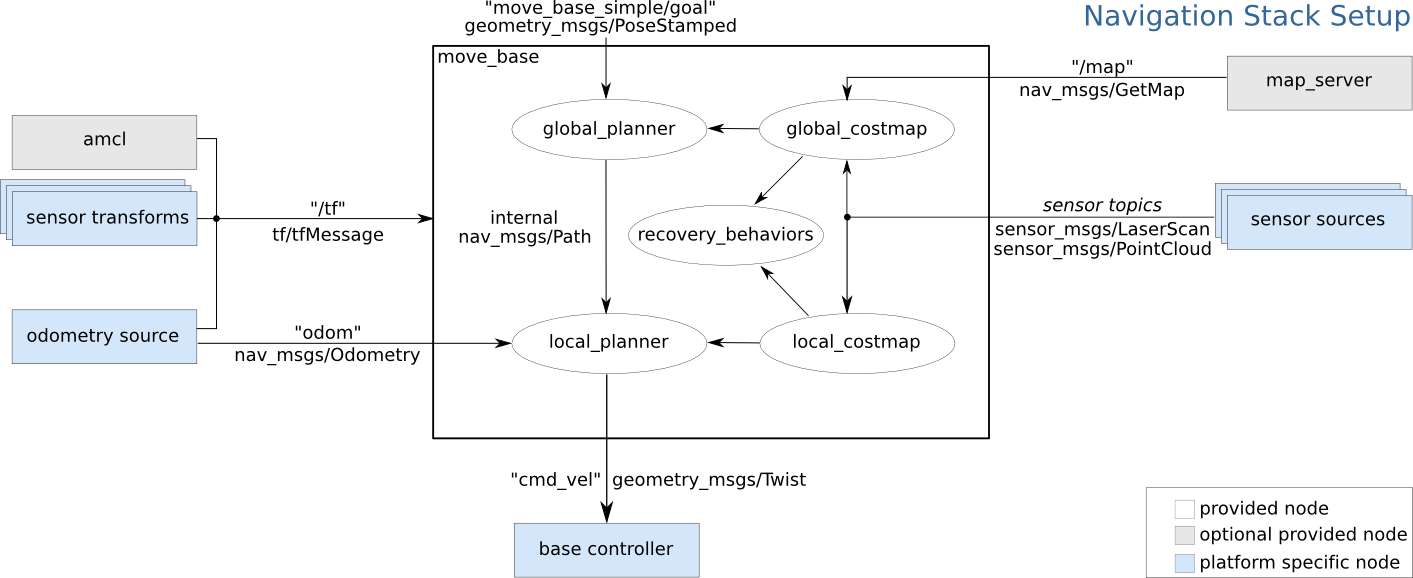
\includegraphics[width=\textwidth]{Pictures/navigation stack setup}
	\caption{recommended navigation stack setup\cite{movebase}}
	
	\label{navigation stack setup}
\end{figure}

The navigation stack has the option to navigate in an existing map by using the combination of the map\_server and amcl (adaptive monte carlo localization). The map\_server publishes a pre recorded map as an occupancy grid. The amcl package then uses that map for localization of the robot by matching the incoming scan result to the map published by the map server. With a good and detail rich map this allows for a accurate estimate of the robots position.\\

For the navigation of a robot the blue squares in the setup need to be supplied, as well as a source for the next goal. In addition every provided node needs to be configured according to the wanted behavior and the mechanical properties of the robot.\\

move\_base has been build very flexible, since it relies on planner plugins and the costmap\_2d package developed by David V. Lu.

This costmap is build in layers, where every layer has a different task and/or inputs. These layers are then combined into the ``master grid''. The master grid is the costmap layer used by the planners to calculate their paths\cite{costmappaper}. By adding additional layers, the navigation considers for example new sensor data or avoids certain sections of the robots environment.

Commonly used data is such produced by range finding sensors like lidar sensors or stereo cameras.\\

The layers provided in the costmap\_2d package are able to mark costs according to the range sensor data and an existing map. These cost can then be inflated by a fixed value radially\cite{costmap} to make a section around obstacles lethal.
\section{navigation2}

navigation2 is the successor of navigation, but is build for ROS2.
Since this thesis aims for a ROS-Noetic solution, the navigation2 stack will not be explored.

\section{Path Planning}

A lot of work has been done regarding path finding. In the navigation\_stack this task has been split into two parts, the global and the local planner.

The global planner is supposed to find a rough path that does not collide with any lethal cells in the costmap. In case of the default package global\_planner of the navigation stack, this is either done using dijkstra or A* algorithms.\\

Since the global planner does not consider the robot directly the local planner is supposed to find a path that is feasible for the dynamics and the steering type of the robot. It also considers the shape of the robot\cite{movebase}.\\



dwa\_local\_planner is according to Kaiyu Zheng the recommended choice for the local planner\cite{navtuningguide}. This planner uses a dynamic window approach, which means the limits of translational and rotational velocities of the robot create a space of feasible trajectories.\\ 
From these possible trajectories a configurable amount will be forward simulated over a given amount of time. These trajectories can be evaluated using configurable weights in combination with the local costmap and the global path.

The ``best'' trajectory is then chosen based on the evaluation. Since the trajectory consist of a combination from translational and rotational velocities these can be used as the input for the motor controller\cite{dwaplanner}.\\

Since the planners of move\_base are implemented in the form of a plugin, not only the plugins of the navigation\_stack are available, but additional ones developed by the ROS community.\\

A popular choice is teb\_local\_planner, which uses the timed elastic band approach, introduced by Christoph Rösmann in his paper about ``Trajectory modification considering dynamic constraints of autonomous robots``.\\
This approach uses the global path as an elastic band, that is repelled by obstacles located next to it and contracted by internal forces like the time constrain.\\
This time constrain is the main difference to the classic elastic band that tries to find the shortest path. At first this seems to be equivalent, since the shortest path should be the fastest but this does not consider the dynamics of the robot itself. 
The dynamics of the robot might prevent it from following the shortest path\cite{Rsmann2012TrajectoryMC}. 

This approach has been implemented in a way, that allows tuning of the individual weights for the deforming forces.\\

The consideration of thy dynamics lets the planner find the ``best'' combination of translational and rotational velocities to send to the motor controller.


\section{ArloBot}
ArloBot is a project of Christen Lofland regarding a Parallax Arlo platform. It consist of a set of ROS packages that allow the robot to navigate and generate a map of a room\cite{chrisl8}.

The navigation of this robot platform is controlled via a web interface, that allows the user to place goals for the robot to drive to, using the navigation stack.

\section{Work of other Carolo-Cup Teams}
In the field of autonomous navigation, a lot of work has been done by all teams that compete in the Carolo-Cup.\\

Unfortunately, this work is often not released to the public, since it would allow other teams to copy an approach giving them an advantage.\\

\section{Summary}
As mentioned, work of other teams in the Carolo-Cup is rarely published. Furthermore it would defeat the purpose of the competition to take the concept of other teams as a reference.\\

The analysis suggest, that the navigation stack is a reasonable choice as a flexible base structure. MoveIt! is more distanced from ROS and rather focused on industrial arm-like robots. It does not seem to be fitting for the scope of this work.\\

Unfortunately the navigation stack does not provide functionality to handle zones that are less preferred. This would be a useful feature to prioritize the right lane of the road. Therefore modifications to the stack are necessary.


There has been a lot of research in path planning of robots. Even for different steering types. The presented solutions to these problems are not bound to a certain use case, which makes them usable in a road environment. 
This thesis mainly focusses on the setup of a working navigation, therefore these planners can be used. The performance of these planners in a road environment are not tested yet. Therfore the development of custom planners for this use case might be necessary in the long term.

All of this covers only the navigation related nodes, but the navigation stack asks for inputs of certain types. The sensor setup is obviously specific to each robot platform. Additionally, to achieve the required navigation behavior, custom data filtering and processing is necessary.


While the project ArloBot of Christen Lofland does not share the same use case, it shares the same robot platform. The project is licensed under the definitions of the MIT License allowing unrestricted usage to any person. Therefore the URDF file of the robot is already existent and will be used as a starting point in this project, although it might need modifications.












